\documentclass[tikz,border=6pt]{standalone}
\usepackage{amsmath}
\usetikzlibrary{positioning,matrix}
\tikzset{
  stencil/.style={minimum size=0.55cm,inner sep=1pt,font=\scriptsize,fill=white},
  central/.style={fill=red!12},
  patch/.style={inner sep=1pt,font=\tiny},
  lab/.style={font=\small,anchor=east},
  head/.style={font=\small\itshape,anchor=south},
}
\begin{document}

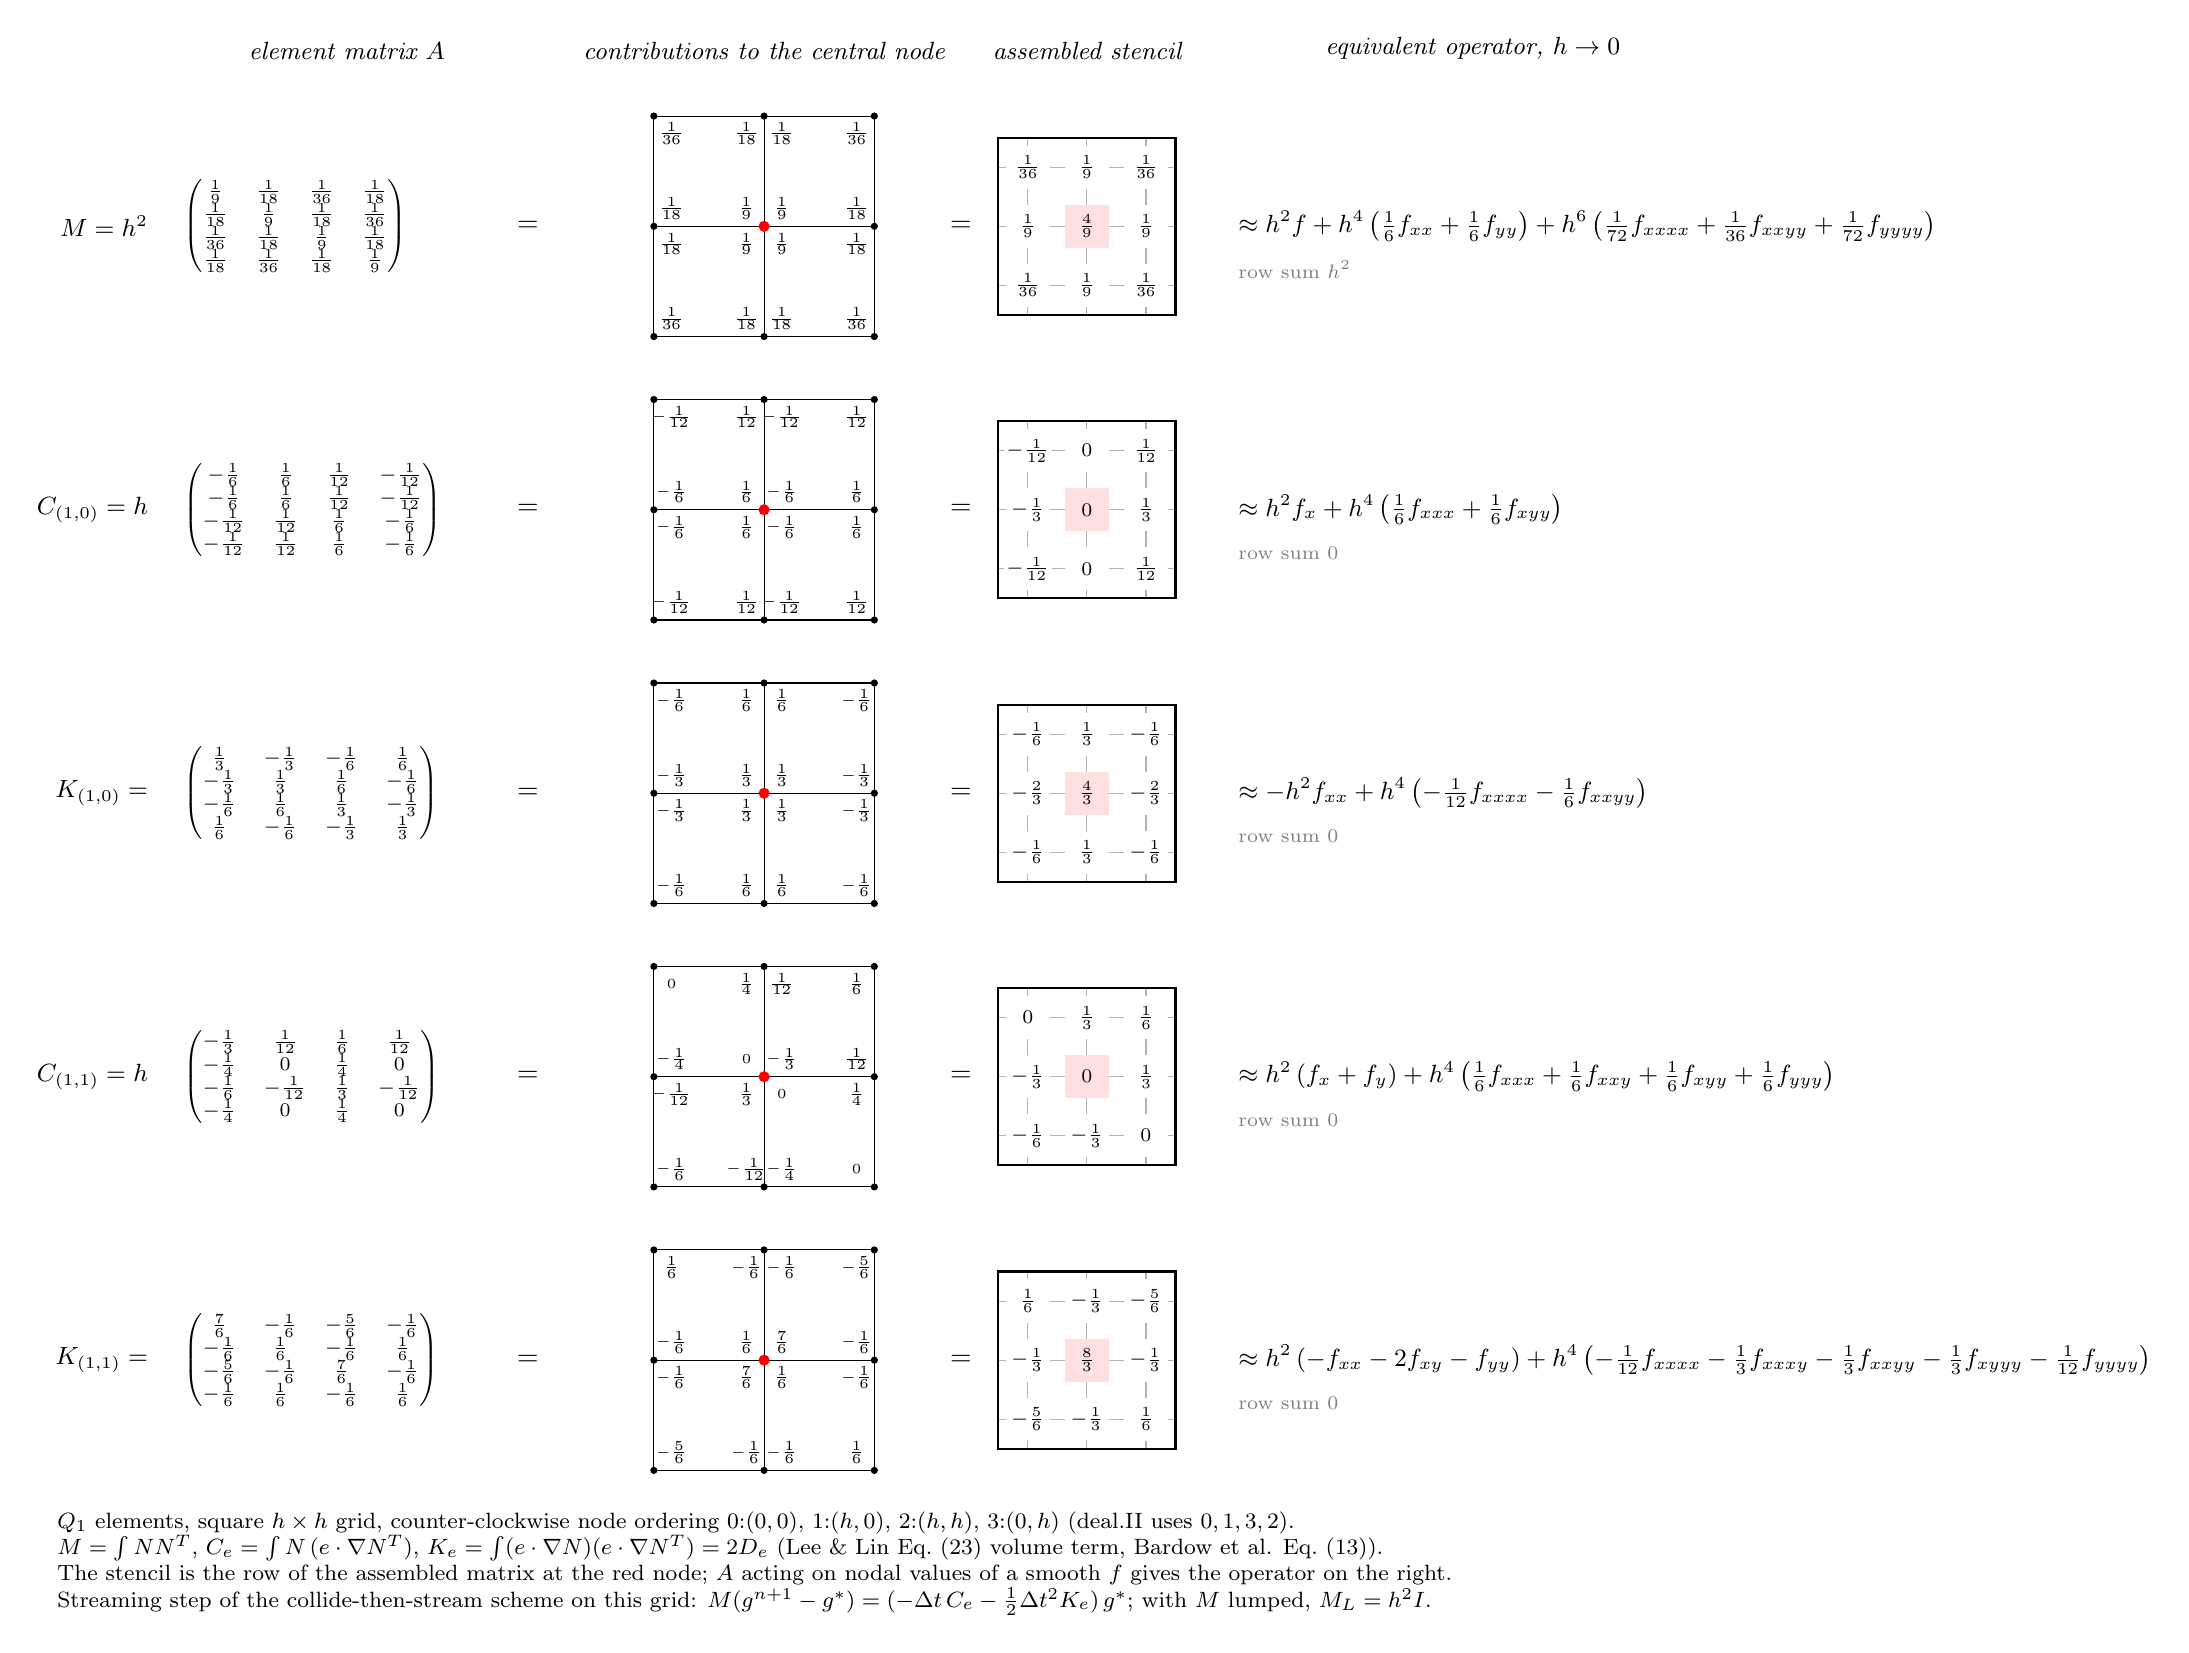
\begin{tikzpicture}
\node[head] at (2.2,2.0) {element matrix $A$};
\node[head] at (7.5,2.0) {contributions to the central node};
\node[head] at (11.6,2.0) {assembled stencil};
\node[head] at (16.5,2.0) {equivalent operator, $h \to 0$};
\node[lab] at (-0.2,0) {$M = h^2$};
\node[anchor=west,font=\scriptsize] at (0,0) {$\begin{pmatrix}\frac{1}{9} & \frac{1}{18} & \frac{1}{36} & \frac{1}{18}\\ \frac{1}{18} & \frac{1}{9} & \frac{1}{18} & \frac{1}{36}\\ \frac{1}{36} & \frac{1}{18} & \frac{1}{9} & \frac{1}{18}\\ \frac{1}{18} & \frac{1}{36} & \frac{1}{18} & \frac{1}{9}\end{pmatrix}$};
\node at (4.5,0) {$=$};
\begin{scope}[shift={(7.5,0)}]
\draw (-1.4,-1.4) rectangle (0.0,0.0);
\node[patch] at (-1.176,-1.176) {$\frac{1}{36}$};
\node[patch] at (-0.22399999999999998,-1.176) {$\frac{1}{18}$};
\node[patch] at (-1.176,-0.22399999999999998) {$\frac{1}{18}$};
\node[patch] at (-0.22399999999999998,-0.22399999999999998) {$\frac{1}{9}$};
\draw (-1.4,0.0) rectangle (0.0,1.4);
\node[patch] at (-1.176,0.22399999999999998) {$\frac{1}{18}$};
\node[patch] at (-0.22399999999999998,0.22399999999999998) {$\frac{1}{9}$};
\node[patch] at (-1.176,1.176) {$\frac{1}{36}$};
\node[patch] at (-0.22399999999999998,1.176) {$\frac{1}{18}$};
\draw (0.0,-1.4) rectangle (1.4,0.0);
\node[patch] at (0.22399999999999998,-1.176) {$\frac{1}{18}$};
\node[patch] at (1.176,-1.176) {$\frac{1}{36}$};
\node[patch] at (0.22399999999999998,-0.22399999999999998) {$\frac{1}{9}$};
\node[patch] at (1.176,-0.22399999999999998) {$\frac{1}{18}$};
\draw (0.0,0.0) rectangle (1.4,1.4);
\node[patch] at (0.22399999999999998,0.22399999999999998) {$\frac{1}{9}$};
\node[patch] at (1.176,0.22399999999999998) {$\frac{1}{18}$};
\node[patch] at (0.22399999999999998,1.176) {$\frac{1}{18}$};
\node[patch] at (1.176,1.176) {$\frac{1}{36}$};
\fill (-1.4,-1.4) circle (1.3pt);
\fill (-1.4,0.0) circle (1.3pt);
\fill (-1.4,1.4) circle (1.3pt);
\fill (0.0,-1.4) circle (1.3pt);
\fill (0.0,0.0) circle (1.3pt);
\fill (0.0,1.4) circle (1.3pt);
\fill (1.4,-1.4) circle (1.3pt);
\fill (1.4,0.0) circle (1.3pt);
\fill (1.4,1.4) circle (1.3pt);
\fill[red] (0,0) circle (2pt);
\end{scope}
\node at (10.0,0) {$=$};
\begin{scope}[shift={(11.6,0)}]
\draw[gray!60] (-1.125,-1.125) grid[step=0.75] (1.125,1.125);
\draw[thick] (-1.125,-1.125) rectangle (1.125,1.125);
\node[stencil] at (-0.75,-0.75) {$\frac{1}{36}$};
\node[stencil] at (-0.75,0.0) {$\frac{1}{9}$};
\node[stencil] at (-0.75,0.75) {$\frac{1}{36}$};
\node[stencil] at (0.0,-0.75) {$\frac{1}{9}$};
\node[stencil,central] at (0.0,0.0) {$\frac{4}{9}$};
\node[stencil] at (0.0,0.75) {$\frac{1}{9}$};
\node[stencil] at (0.75,-0.75) {$\frac{1}{36}$};
\node[stencil] at (0.75,0.0) {$\frac{1}{9}$};
\node[stencil] at (0.75,0.75) {$\frac{1}{36}$};
\end{scope}
\node[anchor=west,font=\small] at (13.4,0) {$\approx h^{2} f + h^{4} \left(\frac{1}{6} f_{xx} + \frac{1}{6} f_{yy}\right) + h^{6} \left(\frac{1}{72} f_{xxxx} + \frac{1}{36} f_{xxyy} + \frac{1}{72} f_{yyyy}\right)$};
\node[anchor=west,font=\scriptsize,gray] at (13.4,-0.55) {row sum $h^{2}$};
\node[lab] at (-0.2,-3.6) {$C_{(1,0)} = h$};
\node[anchor=west,font=\scriptsize] at (0,-3.6) {$\begin{pmatrix}- \frac{1}{6} & \frac{1}{6} & \frac{1}{12} & - \frac{1}{12}\\ - \frac{1}{6} & \frac{1}{6} & \frac{1}{12} & - \frac{1}{12}\\ - \frac{1}{12} & \frac{1}{12} & \frac{1}{6} & - \frac{1}{6}\\ - \frac{1}{12} & \frac{1}{12} & \frac{1}{6} & - \frac{1}{6}\end{pmatrix}$};
\node at (4.5,-3.6) {$=$};
\begin{scope}[shift={(7.5,-3.6)}]
\draw (-1.4,-1.4) rectangle (0.0,0.0);
\node[patch] at (-1.176,-1.176) {$- \frac{1}{12}$};
\node[patch] at (-0.22399999999999998,-1.176) {$\frac{1}{12}$};
\node[patch] at (-1.176,-0.22399999999999998) {$- \frac{1}{6}$};
\node[patch] at (-0.22399999999999998,-0.22399999999999998) {$\frac{1}{6}$};
\draw (-1.4,0.0) rectangle (0.0,1.4);
\node[patch] at (-1.176,0.22399999999999998) {$- \frac{1}{6}$};
\node[patch] at (-0.22399999999999998,0.22399999999999998) {$\frac{1}{6}$};
\node[patch] at (-1.176,1.176) {$- \frac{1}{12}$};
\node[patch] at (-0.22399999999999998,1.176) {$\frac{1}{12}$};
\draw (0.0,-1.4) rectangle (1.4,0.0);
\node[patch] at (0.22399999999999998,-1.176) {$- \frac{1}{12}$};
\node[patch] at (1.176,-1.176) {$\frac{1}{12}$};
\node[patch] at (0.22399999999999998,-0.22399999999999998) {$- \frac{1}{6}$};
\node[patch] at (1.176,-0.22399999999999998) {$\frac{1}{6}$};
\draw (0.0,0.0) rectangle (1.4,1.4);
\node[patch] at (0.22399999999999998,0.22399999999999998) {$- \frac{1}{6}$};
\node[patch] at (1.176,0.22399999999999998) {$\frac{1}{6}$};
\node[patch] at (0.22399999999999998,1.176) {$- \frac{1}{12}$};
\node[patch] at (1.176,1.176) {$\frac{1}{12}$};
\fill (-1.4,-1.4) circle (1.3pt);
\fill (-1.4,0.0) circle (1.3pt);
\fill (-1.4,1.4) circle (1.3pt);
\fill (0.0,-1.4) circle (1.3pt);
\fill (0.0,0.0) circle (1.3pt);
\fill (0.0,1.4) circle (1.3pt);
\fill (1.4,-1.4) circle (1.3pt);
\fill (1.4,0.0) circle (1.3pt);
\fill (1.4,1.4) circle (1.3pt);
\fill[red] (0,0) circle (2pt);
\end{scope}
\node at (10.0,-3.6) {$=$};
\begin{scope}[shift={(11.6,-3.6)}]
\draw[gray!60] (-1.125,-1.125) grid[step=0.75] (1.125,1.125);
\draw[thick] (-1.125,-1.125) rectangle (1.125,1.125);
\node[stencil] at (-0.75,-0.75) {$- \frac{1}{12}$};
\node[stencil] at (-0.75,0.0) {$- \frac{1}{3}$};
\node[stencil] at (-0.75,0.75) {$- \frac{1}{12}$};
\node[stencil] at (0.0,-0.75) {$0$};
\node[stencil,central] at (0.0,0.0) {$0$};
\node[stencil] at (0.0,0.75) {$0$};
\node[stencil] at (0.75,-0.75) {$\frac{1}{12}$};
\node[stencil] at (0.75,0.0) {$\frac{1}{3}$};
\node[stencil] at (0.75,0.75) {$\frac{1}{12}$};
\end{scope}
\node[anchor=west,font=\small] at (13.4,-3.6) {$\approx h^{2} f_{x} + h^{4} \left(\frac{1}{6} f_{xxx} + \frac{1}{6} f_{xyy}\right)$};
\node[anchor=west,font=\scriptsize,gray] at (13.4,-4.15) {row sum $0$};
\node[lab] at (-0.2,-7.2) {$K_{(1,0)} = $};
\node[anchor=west,font=\scriptsize] at (0,-7.2) {$\begin{pmatrix}\frac{1}{3} & - \frac{1}{3} & - \frac{1}{6} & \frac{1}{6}\\ - \frac{1}{3} & \frac{1}{3} & \frac{1}{6} & - \frac{1}{6}\\ - \frac{1}{6} & \frac{1}{6} & \frac{1}{3} & - \frac{1}{3}\\ \frac{1}{6} & - \frac{1}{6} & - \frac{1}{3} & \frac{1}{3}\end{pmatrix}$};
\node at (4.5,-7.2) {$=$};
\begin{scope}[shift={(7.5,-7.2)}]
\draw (-1.4,-1.4) rectangle (0.0,0.0);
\node[patch] at (-1.176,-1.176) {$- \frac{1}{6}$};
\node[patch] at (-0.22399999999999998,-1.176) {$\frac{1}{6}$};
\node[patch] at (-1.176,-0.22399999999999998) {$- \frac{1}{3}$};
\node[patch] at (-0.22399999999999998,-0.22399999999999998) {$\frac{1}{3}$};
\draw (-1.4,0.0) rectangle (0.0,1.4);
\node[patch] at (-1.176,0.22399999999999998) {$- \frac{1}{3}$};
\node[patch] at (-0.22399999999999998,0.22399999999999998) {$\frac{1}{3}$};
\node[patch] at (-1.176,1.176) {$- \frac{1}{6}$};
\node[patch] at (-0.22399999999999998,1.176) {$\frac{1}{6}$};
\draw (0.0,-1.4) rectangle (1.4,0.0);
\node[patch] at (0.22399999999999998,-1.176) {$\frac{1}{6}$};
\node[patch] at (1.176,-1.176) {$- \frac{1}{6}$};
\node[patch] at (0.22399999999999998,-0.22399999999999998) {$\frac{1}{3}$};
\node[patch] at (1.176,-0.22399999999999998) {$- \frac{1}{3}$};
\draw (0.0,0.0) rectangle (1.4,1.4);
\node[patch] at (0.22399999999999998,0.22399999999999998) {$\frac{1}{3}$};
\node[patch] at (1.176,0.22399999999999998) {$- \frac{1}{3}$};
\node[patch] at (0.22399999999999998,1.176) {$\frac{1}{6}$};
\node[patch] at (1.176,1.176) {$- \frac{1}{6}$};
\fill (-1.4,-1.4) circle (1.3pt);
\fill (-1.4,0.0) circle (1.3pt);
\fill (-1.4,1.4) circle (1.3pt);
\fill (0.0,-1.4) circle (1.3pt);
\fill (0.0,0.0) circle (1.3pt);
\fill (0.0,1.4) circle (1.3pt);
\fill (1.4,-1.4) circle (1.3pt);
\fill (1.4,0.0) circle (1.3pt);
\fill (1.4,1.4) circle (1.3pt);
\fill[red] (0,0) circle (2pt);
\end{scope}
\node at (10.0,-7.2) {$=$};
\begin{scope}[shift={(11.6,-7.2)}]
\draw[gray!60] (-1.125,-1.125) grid[step=0.75] (1.125,1.125);
\draw[thick] (-1.125,-1.125) rectangle (1.125,1.125);
\node[stencil] at (-0.75,-0.75) {$- \frac{1}{6}$};
\node[stencil] at (-0.75,0.0) {$- \frac{2}{3}$};
\node[stencil] at (-0.75,0.75) {$- \frac{1}{6}$};
\node[stencil] at (0.0,-0.75) {$\frac{1}{3}$};
\node[stencil,central] at (0.0,0.0) {$\frac{4}{3}$};
\node[stencil] at (0.0,0.75) {$\frac{1}{3}$};
\node[stencil] at (0.75,-0.75) {$- \frac{1}{6}$};
\node[stencil] at (0.75,0.0) {$- \frac{2}{3}$};
\node[stencil] at (0.75,0.75) {$- \frac{1}{6}$};
\end{scope}
\node[anchor=west,font=\small] at (13.4,-7.2) {$\approx -h^{2} f_{xx} + h^{4} \left(- \frac{1}{12} f_{xxxx} -  \frac{1}{6} f_{xxyy}\right)$};
\node[anchor=west,font=\scriptsize,gray] at (13.4,-7.75) {row sum $0$};
\node[lab] at (-0.2,-10.8) {$C_{(1,1)} = h$};
\node[anchor=west,font=\scriptsize] at (0,-10.8) {$\begin{pmatrix}- \frac{1}{3} & \frac{1}{12} & \frac{1}{6} & \frac{1}{12}\\ - \frac{1}{4} & 0 & \frac{1}{4} & 0\\ - \frac{1}{6} & - \frac{1}{12} & \frac{1}{3} & - \frac{1}{12}\\ - \frac{1}{4} & 0 & \frac{1}{4} & 0\end{pmatrix}$};
\node at (4.5,-10.8) {$=$};
\begin{scope}[shift={(7.5,-10.8)}]
\draw (-1.4,-1.4) rectangle (0.0,0.0);
\node[patch] at (-1.176,-1.176) {$- \frac{1}{6}$};
\node[patch] at (-0.22399999999999998,-1.176) {$- \frac{1}{12}$};
\node[patch] at (-1.176,-0.22399999999999998) {$- \frac{1}{12}$};
\node[patch] at (-0.22399999999999998,-0.22399999999999998) {$\frac{1}{3}$};
\draw (-1.4,0.0) rectangle (0.0,1.4);
\node[patch] at (-1.176,0.22399999999999998) {$- \frac{1}{4}$};
\node[patch] at (-0.22399999999999998,0.22399999999999998) {$0$};
\node[patch] at (-1.176,1.176) {$0$};
\node[patch] at (-0.22399999999999998,1.176) {$\frac{1}{4}$};
\draw (0.0,-1.4) rectangle (1.4,0.0);
\node[patch] at (0.22399999999999998,-1.176) {$- \frac{1}{4}$};
\node[patch] at (1.176,-1.176) {$0$};
\node[patch] at (0.22399999999999998,-0.22399999999999998) {$0$};
\node[patch] at (1.176,-0.22399999999999998) {$\frac{1}{4}$};
\draw (0.0,0.0) rectangle (1.4,1.4);
\node[patch] at (0.22399999999999998,0.22399999999999998) {$- \frac{1}{3}$};
\node[patch] at (1.176,0.22399999999999998) {$\frac{1}{12}$};
\node[patch] at (0.22399999999999998,1.176) {$\frac{1}{12}$};
\node[patch] at (1.176,1.176) {$\frac{1}{6}$};
\fill (-1.4,-1.4) circle (1.3pt);
\fill (-1.4,0.0) circle (1.3pt);
\fill (-1.4,1.4) circle (1.3pt);
\fill (0.0,-1.4) circle (1.3pt);
\fill (0.0,0.0) circle (1.3pt);
\fill (0.0,1.4) circle (1.3pt);
\fill (1.4,-1.4) circle (1.3pt);
\fill (1.4,0.0) circle (1.3pt);
\fill (1.4,1.4) circle (1.3pt);
\fill[red] (0,0) circle (2pt);
\end{scope}
\node at (10.0,-10.8) {$=$};
\begin{scope}[shift={(11.6,-10.8)}]
\draw[gray!60] (-1.125,-1.125) grid[step=0.75] (1.125,1.125);
\draw[thick] (-1.125,-1.125) rectangle (1.125,1.125);
\node[stencil] at (-0.75,-0.75) {$- \frac{1}{6}$};
\node[stencil] at (-0.75,0.0) {$- \frac{1}{3}$};
\node[stencil] at (-0.75,0.75) {$0$};
\node[stencil] at (0.0,-0.75) {$- \frac{1}{3}$};
\node[stencil,central] at (0.0,0.0) {$0$};
\node[stencil] at (0.0,0.75) {$\frac{1}{3}$};
\node[stencil] at (0.75,-0.75) {$0$};
\node[stencil] at (0.75,0.0) {$\frac{1}{3}$};
\node[stencil] at (0.75,0.75) {$\frac{1}{6}$};
\end{scope}
\node[anchor=west,font=\small] at (13.4,-10.8) {$\approx h^{2} \left(f_{x} + f_{y}\right) + h^{4} \left(\frac{1}{6} f_{xxx} + \frac{1}{6} f_{xxy} + \frac{1}{6} f_{xyy} + \frac{1}{6} f_{yyy}\right)$};
\node[anchor=west,font=\scriptsize,gray] at (13.4,-11.350000000000001) {row sum $0$};
\node[lab] at (-0.2,-14.4) {$K_{(1,1)} = $};
\node[anchor=west,font=\scriptsize] at (0,-14.4) {$\begin{pmatrix}\frac{7}{6} & - \frac{1}{6} & - \frac{5}{6} & - \frac{1}{6}\\ - \frac{1}{6} & \frac{1}{6} & - \frac{1}{6} & \frac{1}{6}\\ - \frac{5}{6} & - \frac{1}{6} & \frac{7}{6} & - \frac{1}{6}\\ - \frac{1}{6} & \frac{1}{6} & - \frac{1}{6} & \frac{1}{6}\end{pmatrix}$};
\node at (4.5,-14.4) {$=$};
\begin{scope}[shift={(7.5,-14.4)}]
\draw (-1.4,-1.4) rectangle (0.0,0.0);
\node[patch] at (-1.176,-1.176) {$- \frac{5}{6}$};
\node[patch] at (-0.22399999999999998,-1.176) {$- \frac{1}{6}$};
\node[patch] at (-1.176,-0.22399999999999998) {$- \frac{1}{6}$};
\node[patch] at (-0.22399999999999998,-0.22399999999999998) {$\frac{7}{6}$};
\draw (-1.4,0.0) rectangle (0.0,1.4);
\node[patch] at (-1.176,0.22399999999999998) {$- \frac{1}{6}$};
\node[patch] at (-0.22399999999999998,0.22399999999999998) {$\frac{1}{6}$};
\node[patch] at (-1.176,1.176) {$\frac{1}{6}$};
\node[patch] at (-0.22399999999999998,1.176) {$- \frac{1}{6}$};
\draw (0.0,-1.4) rectangle (1.4,0.0);
\node[patch] at (0.22399999999999998,-1.176) {$- \frac{1}{6}$};
\node[patch] at (1.176,-1.176) {$\frac{1}{6}$};
\node[patch] at (0.22399999999999998,-0.22399999999999998) {$\frac{1}{6}$};
\node[patch] at (1.176,-0.22399999999999998) {$- \frac{1}{6}$};
\draw (0.0,0.0) rectangle (1.4,1.4);
\node[patch] at (0.22399999999999998,0.22399999999999998) {$\frac{7}{6}$};
\node[patch] at (1.176,0.22399999999999998) {$- \frac{1}{6}$};
\node[patch] at (0.22399999999999998,1.176) {$- \frac{1}{6}$};
\node[patch] at (1.176,1.176) {$- \frac{5}{6}$};
\fill (-1.4,-1.4) circle (1.3pt);
\fill (-1.4,0.0) circle (1.3pt);
\fill (-1.4,1.4) circle (1.3pt);
\fill (0.0,-1.4) circle (1.3pt);
\fill (0.0,0.0) circle (1.3pt);
\fill (0.0,1.4) circle (1.3pt);
\fill (1.4,-1.4) circle (1.3pt);
\fill (1.4,0.0) circle (1.3pt);
\fill (1.4,1.4) circle (1.3pt);
\fill[red] (0,0) circle (2pt);
\end{scope}
\node at (10.0,-14.4) {$=$};
\begin{scope}[shift={(11.6,-14.4)}]
\draw[gray!60] (-1.125,-1.125) grid[step=0.75] (1.125,1.125);
\draw[thick] (-1.125,-1.125) rectangle (1.125,1.125);
\node[stencil] at (-0.75,-0.75) {$- \frac{5}{6}$};
\node[stencil] at (-0.75,0.0) {$- \frac{1}{3}$};
\node[stencil] at (-0.75,0.75) {$\frac{1}{6}$};
\node[stencil] at (0.0,-0.75) {$- \frac{1}{3}$};
\node[stencil,central] at (0.0,0.0) {$\frac{8}{3}$};
\node[stencil] at (0.0,0.75) {$- \frac{1}{3}$};
\node[stencil] at (0.75,-0.75) {$\frac{1}{6}$};
\node[stencil] at (0.75,0.0) {$- \frac{1}{3}$};
\node[stencil] at (0.75,0.75) {$- \frac{5}{6}$};
\end{scope}
\node[anchor=west,font=\small] at (13.4,-14.4) {$\approx h^{2} \left(-f_{xx} - 2 f_{xy} - f_{yy}\right) + h^{4} \left(- \frac{1}{12} f_{xxxx} -  \frac{1}{3} f_{xxxy} -  \frac{1}{3} f_{xxyy} -  \frac{1}{3} f_{xyyy} -  \frac{1}{12} f_{yyyy}\right)$};
\node[anchor=west,font=\scriptsize,gray] at (13.4,-14.950000000000001) {row sum $0$};
\node[anchor=north west,align=left,font=\footnotesize] at (-1.6,-16.2) {%
$Q_1$ elements, square $h \times h$ grid, counter-clockwise node ordering $0{:}(0,0)$, $1{:}(h,0)$, $2{:}(h,h)$, $3{:}(0,h)$ (deal.II uses $0,1,3,2$).\\
$M = \int N N^T$, $C_e = \int N\,(e\cdot\nabla N^T)$, $K_e = \int (e\cdot\nabla N)(e\cdot\nabla N^T) = 2 D_e$ (Lee \& Lin Eq.~(23) volume term, Bardow et al. Eq.~(13)).\\
The stencil is the row of the assembled matrix at the red node; $A$ acting on nodal values of a smooth $f$ gives the operator on the right.\\
Streaming step of the collide-then-stream scheme on this grid: $M(g^{n+1} - g^*) = (-\Delta t\, C_e - \tfrac12 \Delta t^2 K_e)\, g^*$; with $M$ lumped, $M_L = h^2 I$.};
\end{tikzpicture}
\end{document}